\section{Benutzungsoberfläche}


\subsection{Startfenster}

\begin{figure}[hp] 
  \centering
     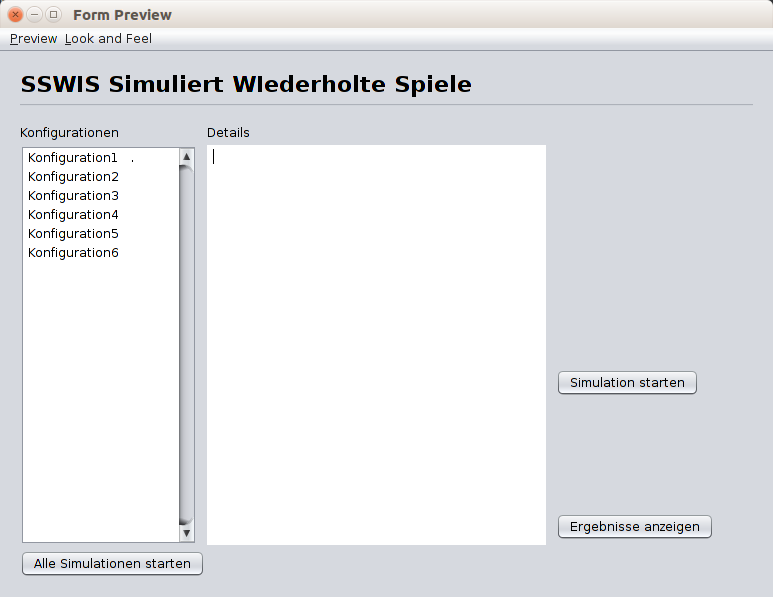
\includegraphics[width=1.1\textwidth]{GUI_Entwurf/Startfenster.png}
  \caption{Hauptfenster}
  \label{fig:Bild1}
\end{figure}

\begin{description}


\item[1. Menü Stufenspiele] Enthält den Menüpunkt 'Stufenspiele verwalten'. Dieser führt zur Stufenspiel Verwaltung.

\item[2. Menü Strategien] Menü enthält den Menüpunkt 'Kombinierte Strategien verwalten'. Dieser führt zu dem Kombinierte Strategien Verwaltung.

\item[3. Menü Initialisierungen] 

\item[4. Menü Konfigurationen] 

\item[5. Menü Ergebnisse] 

\item[6. Liste der Konfigurationen] 

\item[7. Details]

\item[8. Simulation starten] 

\item[9. Ergebnisse anzeigen]

\item[10. Alle Simulationen starten]

\end{description}

\subsection{Stufenspiele Verwaltung}

\begin{figure}[hp] 
  \centering
     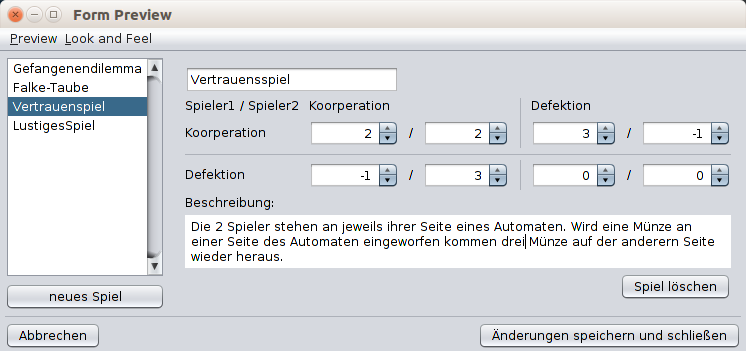
\includegraphics[width=1.1\textwidth]{GUI_Entwurf/SpieleMenue.png}
  \caption{Stufenspiel Verwaltung}
  \label{fig:Bild1}
\end{figure}

\begin{description}

\item[1. Liste] 

\item[2. Name] 

\item[3. Auszahlungen] 

\item[4. Beschreibung] 

\item[5. neues Spiel] 

\item[6. Spiel löschen] 

\item[7. Abbrechen] 

\item[8. Änderungen speichern und schließen] 

\end{description}

\pagebreak

\subsection{Kombinierte Strategien Verwaltung}

\begin{figure}[hp] 
  \centering
     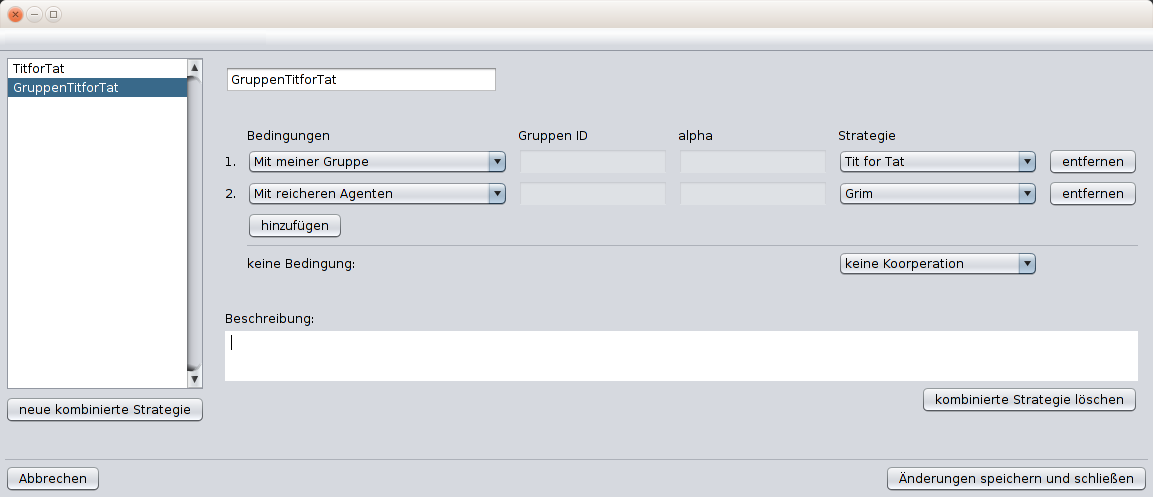
\includegraphics[width=1.1\textwidth]{GUI_Entwurf/StrategienMenue.png}
  \caption{Kombinierte Strategien Verwaltung}
  \label{fig:Bild1}
\end{figure}

\begin{description}

\item[1. Liste] 

\item[2. Name] 

\item[3. Nummerierung] 

\item[4. Bedingung] 

\item[5. Gruppen ID] 

\item[6. alpha] 

\item[7. Strategie] 

\item[8. entfernen] 

\item[9. hinzufügen] 

\item[10. keine Bedingung] 

\item[11. Beschreibung] 

\item[12. neue kombinierte Strategie] 

\item[13. kombinierte Strategie löschen] 

\item[14. Abbrechen] 

\item[15. Änderungen speichern und schließen] 

\end{description}

\pagebreak

\subsection{Initialisierung erstellen}

\begin{figure}[hp] 
  \centering
     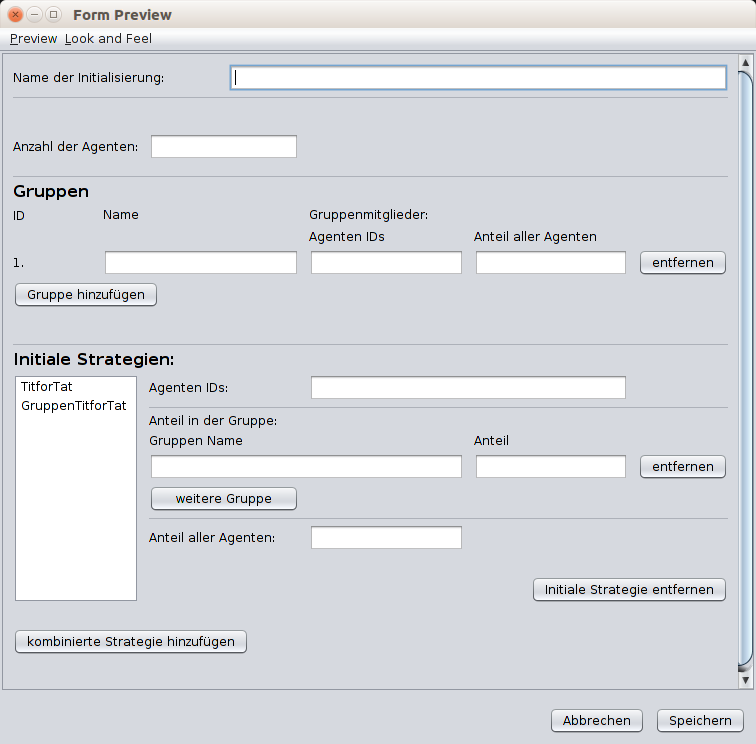
\includegraphics[width=1.1\textwidth]{GUI_Entwurf/NeueInitialisierung.png}
  \caption{Initialisierung}
  \label{fig:Bild1}
\end{figure}


\begin{description}

\item[1. Name] 

\item[2. Anzahl der Agenten] 

\item[3. Gruppen - ID] 

\item[4. Gruppen - Name] 

\item[5. Gruppen - AgentenIDs] 

\item[6. Gruppen - Anteil aller Agenten] 

\item[7. Gruppen - entfernen] 

\item[8. Gruppen - Gruppe hinzufügen] 

\item[9. Initiale Strategien - Liste] 

\item[10. Initiale Strategien - Agenten IDs] 

\item[11. Initiale Strategien - Gruppen Name] 

\item[12. Initiale Strategien - Anteil] 

\item[13. Initiale Strategien - entfernen] 

\item[14. Initiale Strategien - weitere Gruppe] 

\item[15. Initiale Strategien - Anteil der Agenten] 

\item[16. Initiale Strategien - kombinierte Strategie hinzufügen] 

\item[17. Abbrechen] 

\item[18. Speichern] 

\end{description}


\pagebreak

\subsection{Konfigurationen erstellen}

\begin{figure}[hp] 
  \centering
     \includegraphics[width=1.0\textwidth]{GUI_Entwurf/.png}
  \caption{Konfiguration}
  \label{fig:Bild2}
\end{figure}

\begin{description}

\item[1. ] 

\item[2. ] 

\item[3. ] 

\item[4. ] 

\item[5. ] 

\item[6. ] 

\item[7. ] 

\item[8. ] 

\item[9. ] 

\item[10. ] 

\end{description}

\pagebreak


\subsection{Ergebnisse anzeigen}

\begin{figure}[hp] 
  \centering
     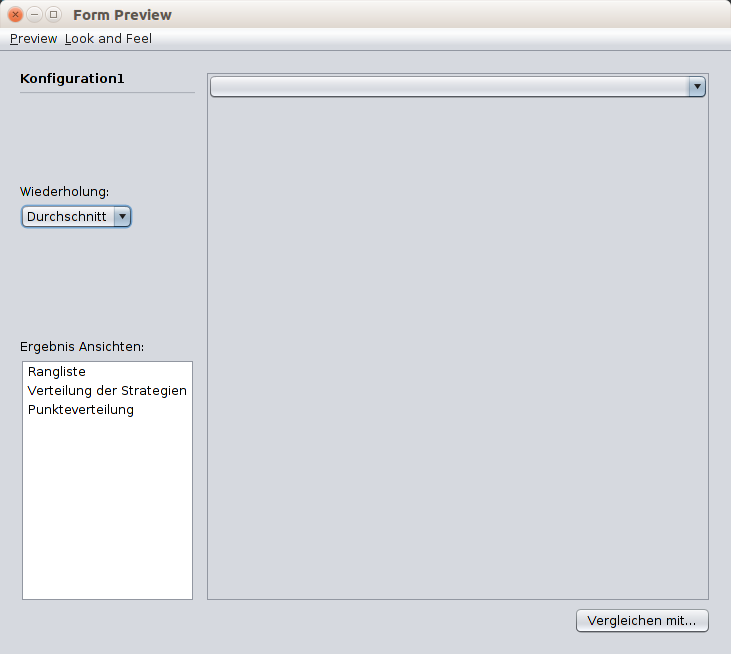
\includegraphics[width=1.1\textwidth]{GUI_Entwurf/Ergebnisfenster(1).png}
  \caption{Ergebnisfenster}
  \label{fig:Bild7}
\end{figure}

\begin{description}

\item[1. ] 

\item[2. ] 

\item[3. ] 

\item[4. ] 

\item[5. ] 

\item[6. ] 

\item[7. ] 

\item[8. ] 

\item[9. ] 

\item[10. ] 

\end{description}

\pagebreak


\subsection{Ergebnisse vergleichen}

\begin{figure}[hp] 
  \centering
     \includegraphics[width=1.1\textwidth]{GUI_Entwurf/.png}
  \caption{Vergleichenfenster}
  \label{fig:Bild1}
\end{figure}

\begin{description}

\item[1. ] 

\item[2. ] 

\item[3. ] 

\item[4. ] 

\item[5. ] 

\item[6. ] 

\item[7. ] 

\item[8. ] 

\item[9. ] 

\item[10. ] 

\end{description}



